\documentclass{slide}

\usepackage{changepage}
\usepackage{tabto}
% \usepackage{pgfpages}
% \setbeameroption{show notes on second screen}

\title{Microservices Architecture}
\subtitle{CSSE6400}
\author{Richard Thomas}
\date{\week{7}}

\begin{document}

\maketitle

\point[Microservices]{Inspired by DDD}

\definition{Bounded Context}{Logical boundary of a domain where particular terms and rules apply consistently.}

\image[height=.97\textheight]{diagrams/bounded-context.png}

\image[height=.96\textheight]{diagrams/microservices-arch.png}

\point[Choreography \& Orchestration]{
\begin{description}
    \item[Choreography] Similar to event-driven \highlight{broker}
    \item[Orchestration] Similar to event-driven \highlight{mediator}
\end{description}
}

\begin{frame}
    \begin{adjustwidth}{-10mm}{-10mm}
        \centering
        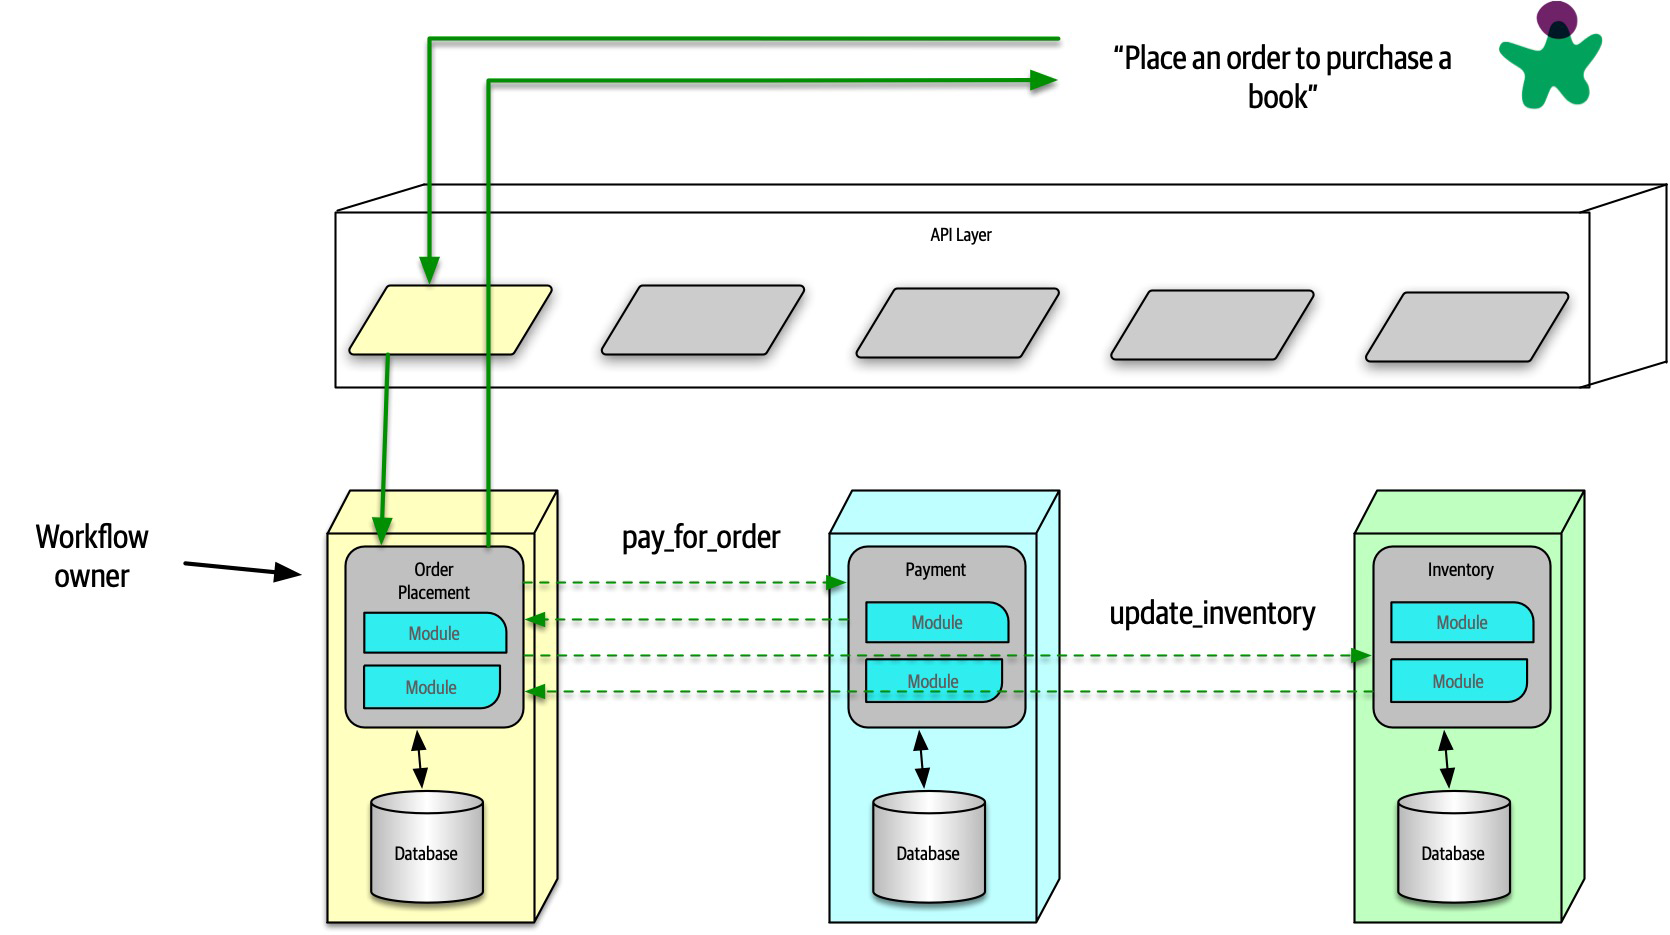
\includegraphics[width=0.96\paperwidth]{diagrams/choreography.png}
    \end{adjustwidth}
\end{frame}

\image[height=.98\textheight]{diagrams/orchestration.png}

\begin{frame}{Pros \& Cons}
    \vspace{1mm}
    {\LARGE
    \begin{description}
        \item[Modularity] \tabto{15em}
\includegraphics[width=8mm]{../../shared/images/thumbs-up.png}
        \item[Extensibility] \tabto{15em}
\includegraphics[width=8mm]{../../shared/images/thumbs-up.png}
        \item[Reliability] \tabto{15em}
\includegraphics[width=8mm]{../../shared/images/thumbs-up.png}
        \item[Interoperability] \tabto{15em}
\includegraphics[width=8mm]{../../shared/images/thumbs-up.png}
        \item[Scalability] \tabto{15em}
\includegraphics[width=8mm]{../../shared/images/thumbs-up.png}
        \item[Security] \tabto{15em}
\includegraphics[trim=57 145 70 85,clip,width=8mm]{../../shared/images/neutral.png}
        \item[Deployability] \tabto{15em}
\includegraphics[trim=22 19 22 12,clip,width=8mm]{../../shared/images/neutral.png}
        \item[Testability] \tabto{15em}
\includegraphics[trim=22 19 22 12,clip,width=8mm]{../../shared/images/neutral.png}
        \item[Simplicity] \tabto{15em}
\includegraphics[trim=22 19 22 12,clip,width=8mm]{../../shared/images/thumbs-down.png}
    \end{description}
    }
\end{frame}

\end{document}